\documentclass[oneside, 12pt]{book}
\usepackage[utf8]{inputenc}
\usepackage{geometry}
\usepackage{graphicx}
\usepackage{amsmath}
\usepackage{amssymb}
\usepackage{tikz}
\usepackage{color}
\usepackage{hyperref}
\hypersetup{
    colorlinks=false, %set true if you want colored links
    linktoc=all,     %set to all if you want both sections and subsections linked
}
\usetikzlibrary{automata, positioning, arrows}

\tikzset{
->, % makes the edges directed
>=stealth', % makes the arrow heads bold
node distance=3cm, % specifies the minimum distance between two nodes. Change if necessary.
every state/.style={thick}, % sets the properties for each ’state’ node
initial text=$ $, % sets the text that appears on the start arrow
}
\graphicspath{ {./images/} }
\newtheorem{theorem}{Theorem}
\title{
  Automata and Languages
}

\author{Pranav Wadhwa}
\begin{document}
\maketitle
\tableofcontents
\chapter{Regular Languages}

\section{Terms}

\subsection{Alphabet}
Alphabet is a non-empty finite set. Example: $\Sigma = \{0,1\}, \Gamma=\{0,1,x,y,z\}$

\subsection{String}
String is a finite sequence of symbols from an alphabet. There are \textbf{countably infinite} strings.

\section{Decision Problems}

Decision Problems is a function which takes an input string and decides whether to accept it or not.

\emph{input}: string (finite length sequence from some finite alphabet $\Sigma$)

\emph{output}: accept or reject, true or false, 1 or 0

A decision problem is specified by a function: strings $\to$ boolean

A decision problem is equivalently specified by a subset of strings
$w\in S \iff f(w) = $ accept\\

\textbf{Cardinality}
Each string is finite

There are countably infinite strings

There are uncountably infinite decision problems (subset of strings).

There are countably infinite finite automata, regular expressions, and regular language.


\section{Finite Automaton}

\textbf{Definition}: A finite automaton $M$ is defined by a 5-tuple $M=(Q,\Sigma, \delta, q_{0},F)$ where

$Q$ is finite set of State

$\Sigma$ is the finite alphabet

$\delta: Q\times \Sigma\to Q$ is transition function

$q_{0}\in Q$ is the start state

$F\subseteq Q$ is the set of accept state (this may be empty)

Example:

Consider $M$ definied by:
$Q=\{q_{0}, q_{1}, q_{2}\}$

$\Sigma=\{0,1\}$

$q_{0} is the start state$

$F=\{q_{1}\}$

Since $Q$ and $\Sigma$ finite, $\delta$ can be defined by a finite state transition table:

\begin{center}
  \begin{tabular}{| c | c |c | }
    \hline
     & 0 & 1\\
    \hline
    $q_{0}$ & $q_{0}$ & $q_{1}$\\
    $q_{1}$ & $q_{2}$ & $q_{1}$\\
    $q_{2}$ & $q_{1}$ & $q_{1}$\\
    \hline
  \end{tabular}
\end{center}


\emph{State Diagram}:

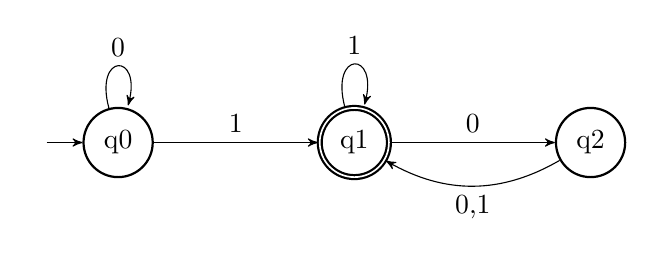
\begin{tikzpicture}
  \node[state, initial] (0) {q0};
  \node[state, right of=0, accepting] (1) {q1};
  \node[state, right of=1] (2) {q2};


  \draw (0) edge[loop above] node{0} (0)
  (0) edge[above] node{1} (1)
  (1) edge[loop above] node{1} (1)
  (1) edge[above] node{0} (2)
  (2) edge[bend left, below] node{0,1} (1);
\end{tikzpicture}


\subsection{Definition of Computation}

Given a finite automaton $M=(Q,\Sigma, \delta, q_{0}, F)$ and input string $w=\sigma_{q}\sigma_{2}\dots \sigma_{n}$.

Let a configuration be a $c\in Q$.

Define the execution of $M$ on $w$ to eb the nuique sequence of configs $c_{0}c_{1},\dots,c_{n}$ s.t $c_{0}=q_{0}, c_{i+1}=\delta(c_{i}, \sigma_{i+1})$ for $i=0\dots n-1$.

If $c_{n}\in F$, then we say that $M$ accepts $w$, else it rejects $w$.

\emph{Reconsider Example}:
Consider the execution of the previous finite automaton $M$ on a few examples

$1111$: $q_{0}\stackrel{1}{\to}q_{1}\stackrel{1}{\to}q_{1}\stackrel{1}{\to}q_{1}\stackrel{1}{\to}q_{1}$ accept

$1110$:
$q_{0}\stackrel{1}{\to}q_{1}\stackrel{1}{\to}q_{1}\stackrel{1}{\to}q_{1}\stackrel{0}{\to}q_{2}$ reject
This above program accepts even number of $0s$ (or no $0$) after last $1$.

\section{Languages}

A \emph{language} is a subset of strings

Examples: $\emptyset$

all strings over $\Sigma = \{0,1\}$

strings with more 1s than 0s etc


A machine is said to \emph{accept} a string and \emph{recognize} a language.

\textbf{Definition} $M$ \emph{recognizes} the language $A$ iff $A=\{w:M\text{ accepts } w\}$


\textbf{Definition} A langauge is called \emph{regular} iff some finite automaton $M$ recognizes it.

\emph{Note}
\begin{itemize}
  \item For any regular langauge there are infinitely many finite automate that recogize it.
  \item For any ffinite automaton $M$, there is only one language it.
\end{itemize}



\section{Regular operations on Languages}
Let $A$ and $B$ be languages. The regular operations on languages are:

complement $\bar{A} = \{w:w\notin A\}$

intersection $A\cap B = \{w: w\in A \text{ and } w\in B\}$

union $A\cup B = \{w: w\in A \text{ or } w\in B\}$

concatenation $A\circ B = \{wx: w\in A \text{ and } x\in B\}$

star $A^{*}=\{w_{1}w_{2}\dots w_{k}: k\ge 0 \text{ and each } w_{i} \in A \}$



\begin{theorem}
  The class of regular languages is closed under complement
\end{theorem}

\emph{Intuition}: When you have a finite automata $M$ which recognize a langauge $L$ then $\bar{L}$ is also regular and we can get a finite automata $\bar{M}$ which same as $M$ but has the accept and reject states flipped

\begin{theorem}
  The class of regular langauge is closed uner intersection and union.
\end{theorem}

\emph{Intuition/Hint}: Let 2 regular language be $L_{1}$ and $L_{2}$ which have state machines $M_{1}$ and $M_{2}$. Let $M=(Q,\Sigma, \delta, q_{0}, F)$ where:

\begin{itemize}
  \item $Q=Q_{1}\times Q_{2}$
  \item $q_{0} = (q_{01}, q_{02})$
  \item $\delta((q_{1}, q_{2}), a) = (\delta_{1}(q_{1}, a), \delta_{2}(q_{2}, a))$
\end{itemize}

Example on how to do the intersection operation.

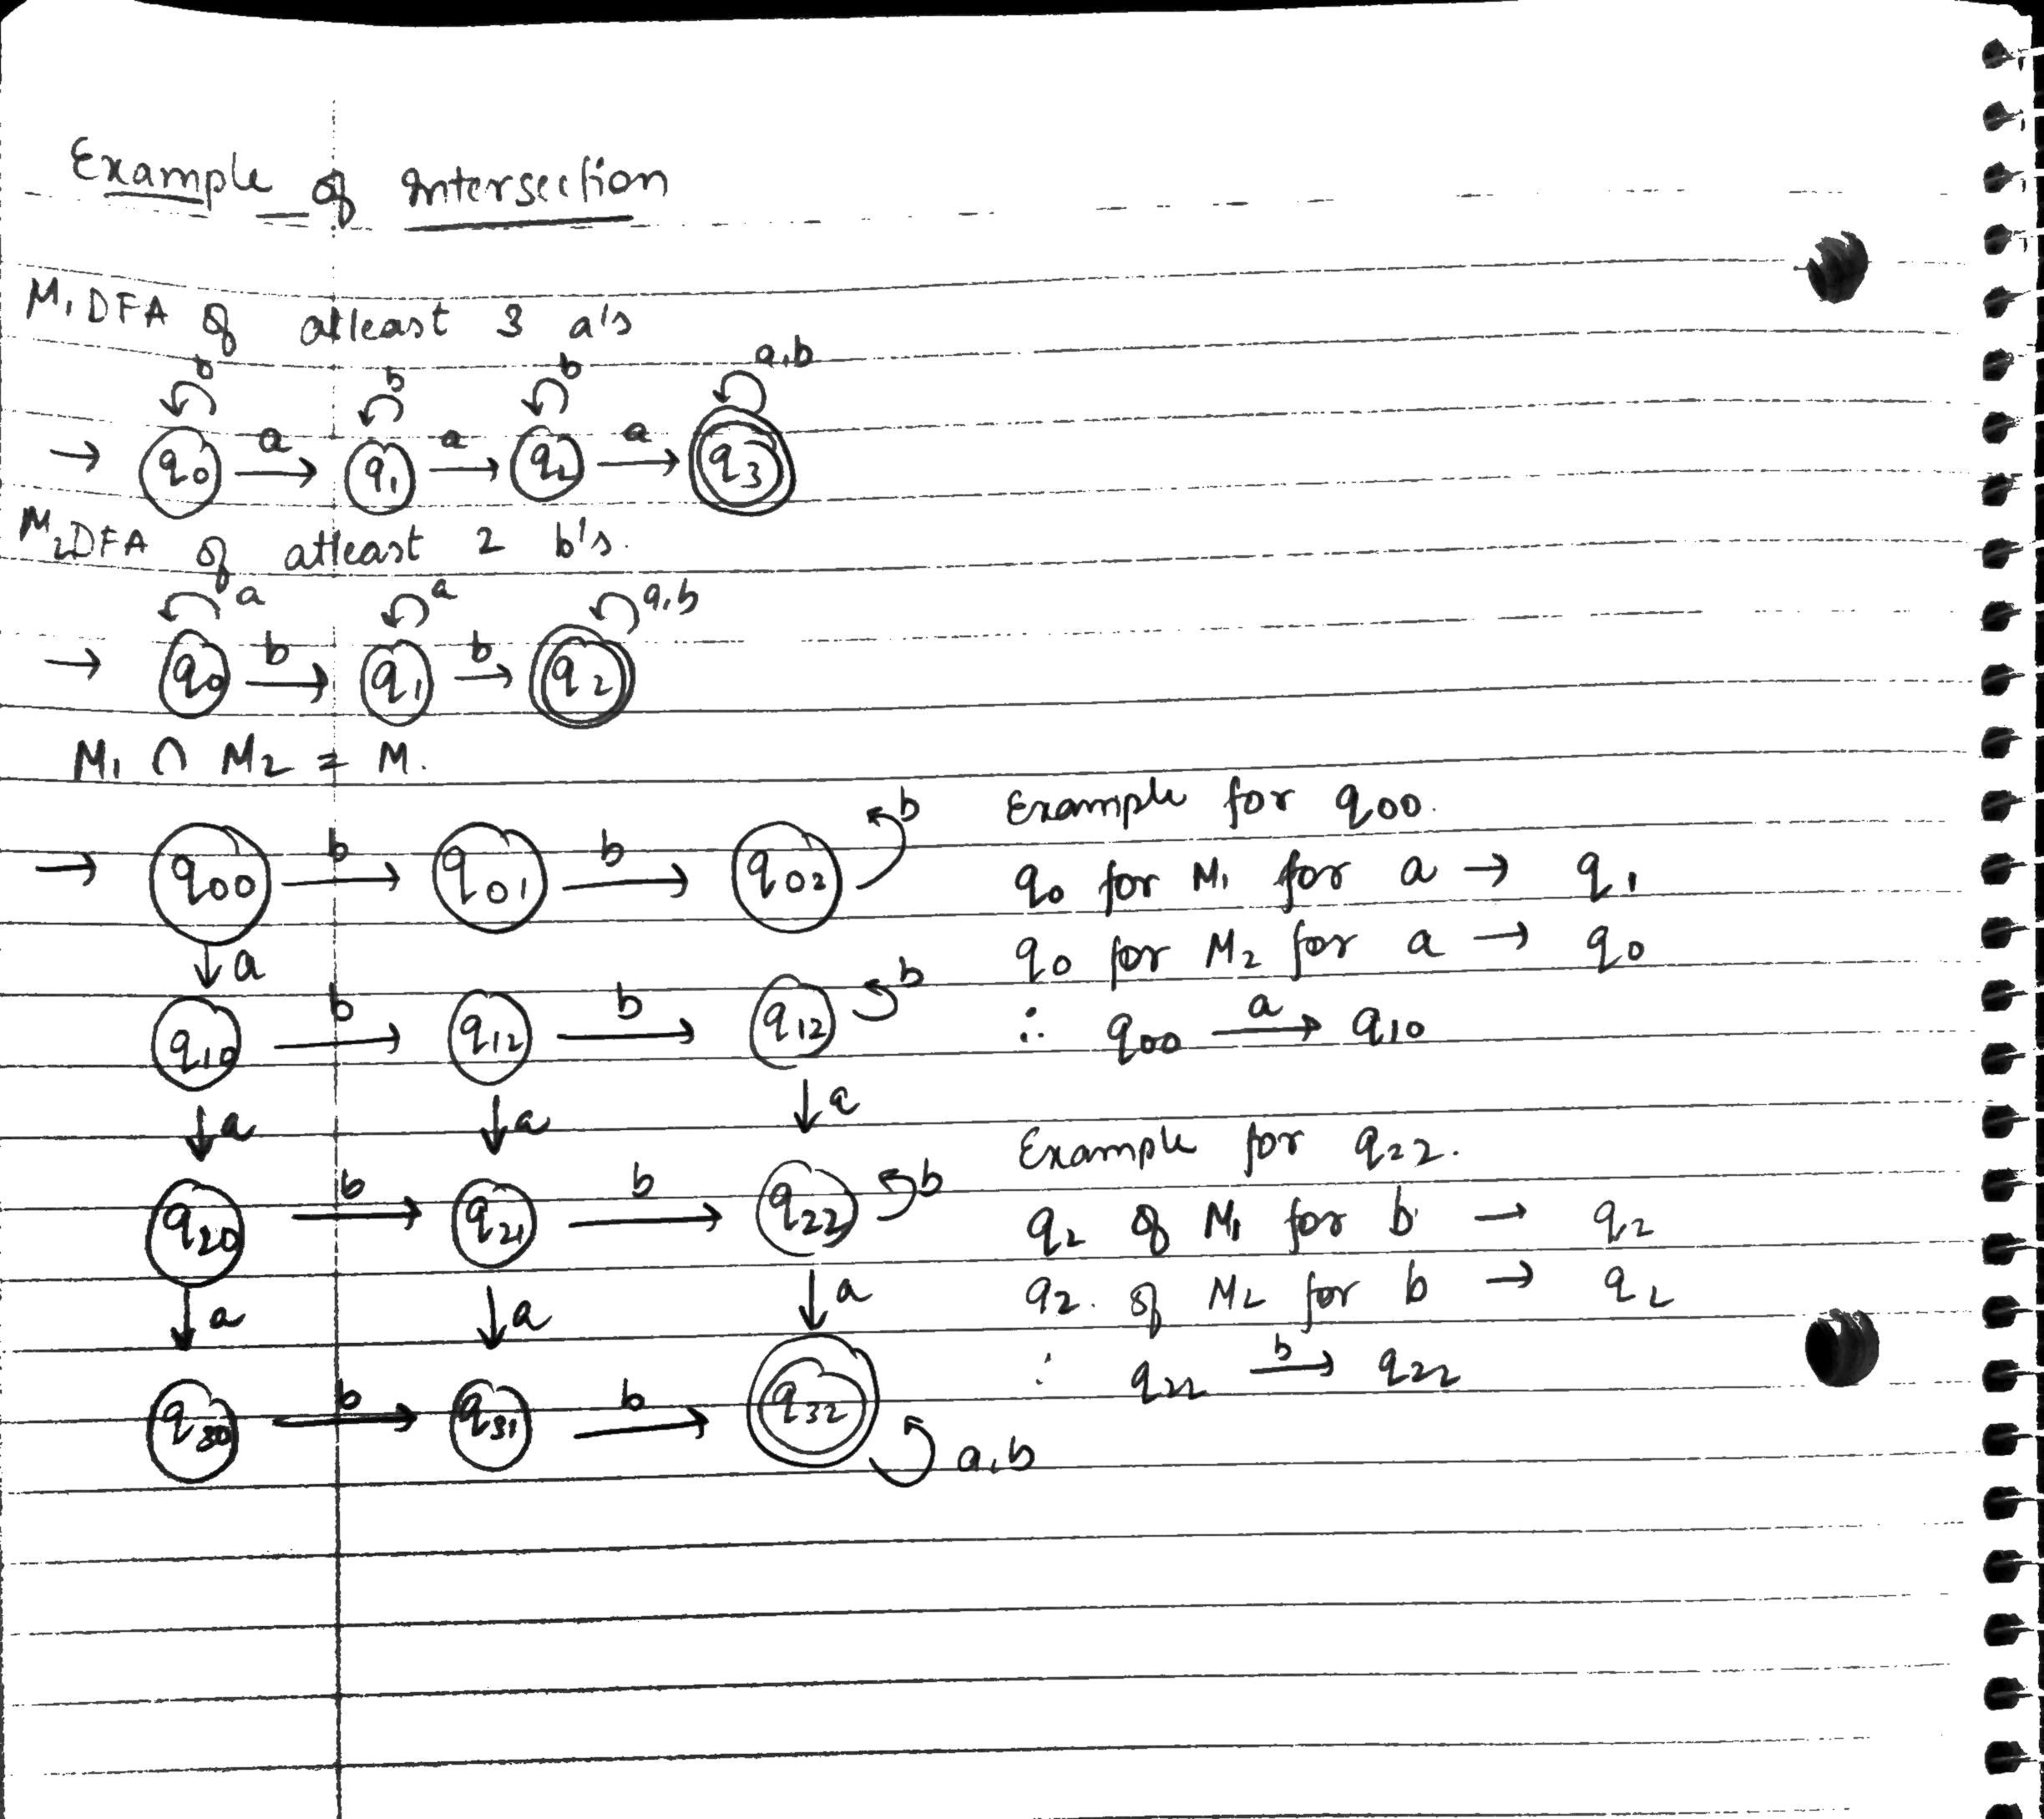
\includegraphics[width=\textwidth]{intersection}

\section{Nondeterministic finite automata}

\textbf{Definition} A \emph{nondeterministic finite automaton} (NFA) is defined by a 5-tuple $M=(Q,\Sigma, \delta, q_{0}, F)$ where:

$Q$ is the finite set of states

$\Sigma$ is the finite alphabet

$\delta: Q\times \Sigma_{\lambda}\to \mathcal{P}(Q)$ is the transition relation (i.e $\delta(q, \sigma)\subseteq Q$)

$q_{0}\in Q$ is start state

$F\subseteq Q$ is set of accept states

where we let $\lambda$ denote the null character, and let $\Sigma_{\lambda} = \Sigma\cup \{\lambda\}$, which will allow spontaneous state transitions that do not process the next input symbol.

\emph{Note} Difference from DFA is the NFA allows multiple next possible state for one input.

\textbf{Example} Consider $M$ defined by

$Q = \{q_{0}, q_{1}, q_{2}, q_{3}\}$

$\Sigma = \{0,1\}$

$q_{0} = q_{0}$

$F=\{q_{3}\}$

\begin{center}
  \begin{tabular}{| c| c| c| c| }
    \hline
    & 0 & 1 & $\lambda$\\
    \hline
    $q_{0}$ & $\{q_{0}\}$ & $\{q_{0}, q_{1}\}$ & $\emptyset$\\
    $q_{1}$ & $\{q_{2}\}$ & $\emptyset$ & $\{q_{2}\}$\\
    $q_{2}$ & $\emptyset$ & $\{q_{3}\}$ & $\emptyset$\\
    $q_{3}$ & $\{q_{3}\}$ & $\{q_{3}\}$ & $\emptyset$\\
    \hline
  \end{tabular}
\end{center}

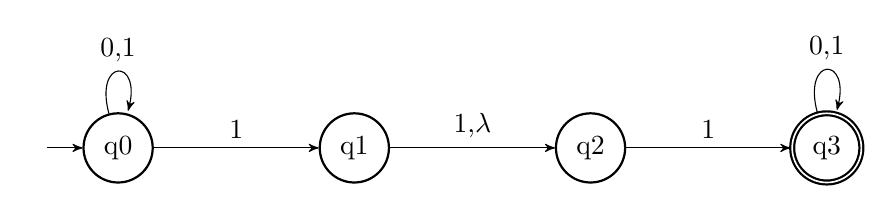
\begin{tikzpicture}
  \node[state, initial] (0) {q0};
  \node[state, right of=0] (1) {q1};
  \node[state, right of=1] (2) {q2};
  \node[state, right of=2, accepting] (3) {q3};


  \draw (0) edge[loop above] node{0,1} (0)
  (0) edge[above] node{1} (1)
  (1) edge[above] node{1,$\lambda$} (2)
  (2) edge[above] node{1} (3)
  (3) edge[loop above] node{0,1} (3);
\end{tikzpicture}

In this example, $M$ accepts strings containing 11 or 101 as a substring.

\subsection{Definition of nondeterministic computation}

Instead of a sequence of configurations, we consider a tree of possible configurations.

Given an NFA $M = (Q,\Sigma,\delta, q_{0}, F)$ and input string $w = \delta_{1}\delta_{2}\dots \delta_{n} \text{ for } \delta_{i} \in \Sigma$.

Define a \emph{configuration} be $c=(q, i)$ s.t $q\in Q$ and $i$ is position of last input symbol read.

Define the \emph{execution tree} of $M$ on $w$ to be the directed tree rooted at $c = (q_{0}, 0)$ s.t there is an edge $c=(q, i)$ to $\bar{c}=(\bar{q},\bar{i})$

We sau tht $M$ accepts $w$ if the execution tree contains a configuration $(q,n)$ such that $q\in F$, else it rejects $w$.


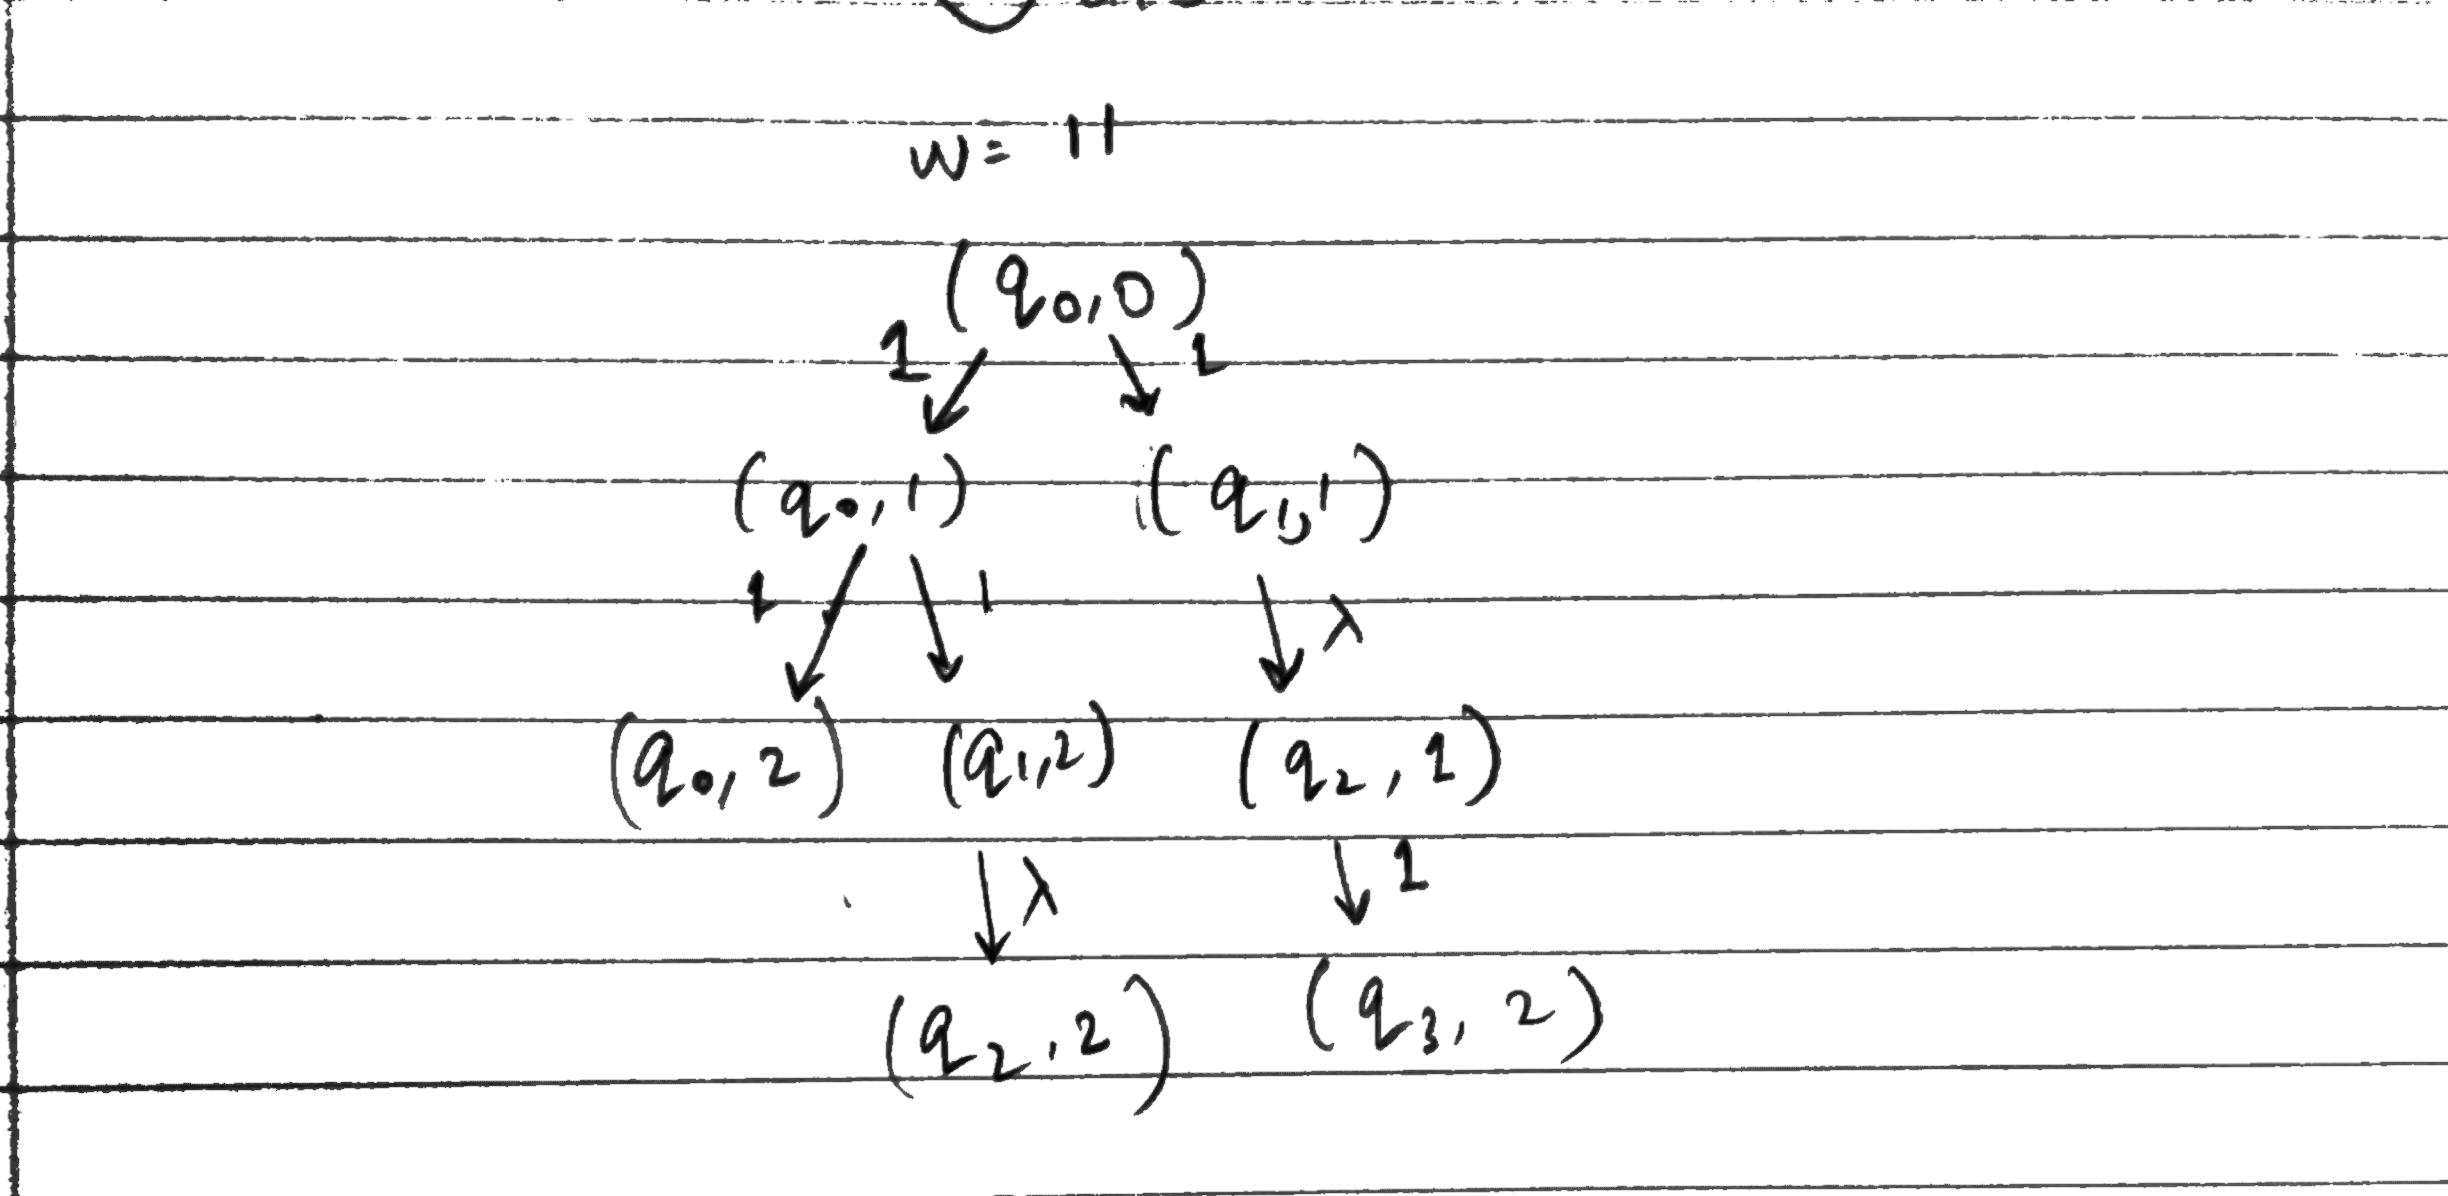
\includegraphics[width=\textwidth]{tree}
\begin{center}
\emph{Example of execution tree on input $w=11$ for machine $M$ defined above}
\end{center}

\section{NFA and DFA}

\begin{theorem}

Every NFA $M$ has an equivalent DFA $\bar{M}$.
\end{theorem}

\textbf{Corollary} A language is regular $\leftrightarrow$ some NFA recogizes it
($\leftrightarrow$ some DFA recognizes it)


\section{Regular Operations on Language}

\begin{theorem}
The class of regular langauges is closed under union.
\end{theorem}

\textbf{Construct}:

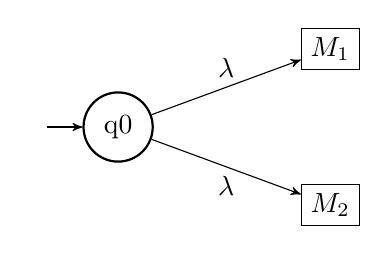
\begin{tikzpicture}
  \node[state, initial] (0) {q0};
  \node[rectangle, draw=black, above right=0.4cm and 2cm of 0] (1) {$M_{1}$};
  \node[rectangle, draw=black, below right=0.4cm and 2cm of 0] (2) {$M_{2}$};

  \draw (0) edge[above] node{$\lambda$} (1)
  (0) edge[below] node{$\lambda$} (2);

\end{tikzpicture}


\begin{theorem}
The class of regular languages is closed under concatenation
\end{theorem}

\textbf{Context}


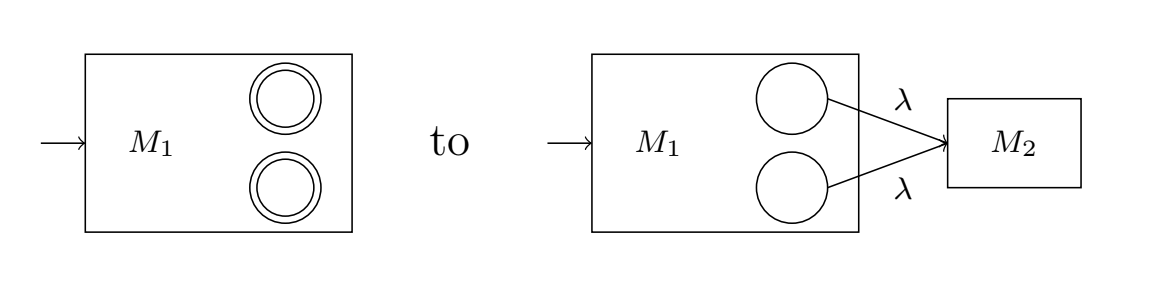
\includegraphics[width=\textwidth]{concat}


\begin{theorem}
This class of regular languages is closed under star.
\end{theorem}
\textbf{Context}

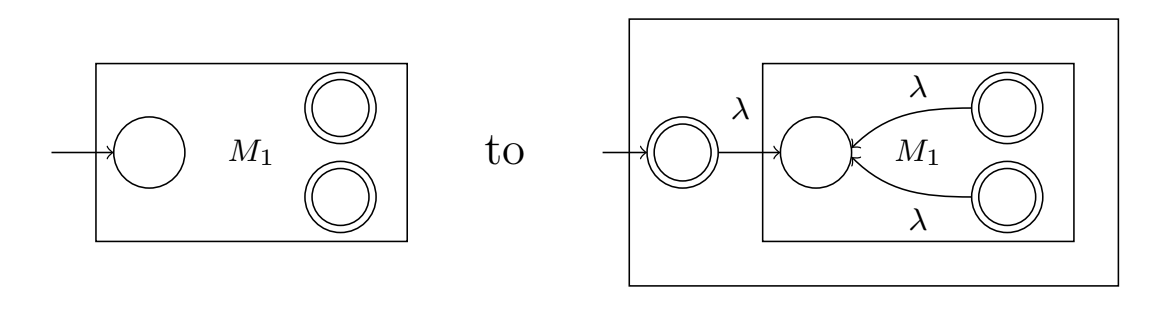
\includegraphics[width=\textwidth]{star}


\section{Regular Expression}

A meta language for specifying decision problems over strings
i.e a meta language for specifing a language

\textbf{Definition} $R$ is a regular expression if

$R = a$ for some $a$ in $\Sigma$

$R=\epsilon$

$R=\emptyset$

$R = R_{1}\cup R_{2}$

$R = R_{1}R_{2}$

$R = R_{1}^{*}$

$R = (R_{1})$

\textbf{Additionaly}
\begin{itemize}
  \item Precedence: $*, \circ, \cup$
  \item For a regular expression $R$, $L(R)$ denotes it language
\end{itemize}

\textbf{Important Examples}

$\Sigma = \{0,1\}$

\begin{itemize}
  \item $L(0\cup 1) = \{0,1\}$
  \item $L((0\cup 1)^{*}) =$ all strings over $\{0,1\}$
        \item $L((\Sigma \Sigma)^{*})=$ strings of even length
\end{itemize}


\textbf{Identities}

\begin{itemize}
  \item $R\cup \emptyset = R$
  \item $R\epsilon = R$
  \item $R\cup \epsilon \neq R$
  \item $R\emptyset \neq R$
\end{itemize}

\begin{theorem}
  A language $L$ is regular $\leftrightarrow$ exists a regular expression $R$ such that $L(R) = R$
  \begin{itemize}
    \item Any decision problem that can be specified by an RE can be solved by an FA
    \item Any decision problem that can be implemented by an FA can be specified by an RE
  \end{itemize}
\end{theorem}

\textbf{Regular Expression to NFA}

if $R = a$ then NFA

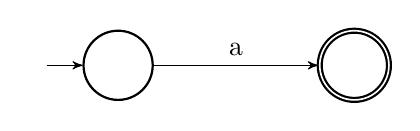
\begin{tikzpicture}
  \node[state, initial] (q1) { };
  \node[state, accepting, right of=q1] (q2) {  };

  \draw (q1) edge[above] node{a} (q2);
\end{tikzpicture}

if $R = \epsilon$ then NFA


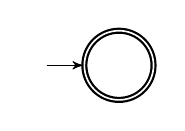
\begin{tikzpicture}
  \node[state, initial, accepting] (q1) { };

\end{tikzpicture}


if $R = \emptyset$ then NFA

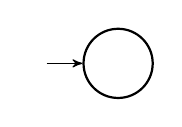
\begin{tikzpicture}
  \node[state, initial] (q1) { };
\end{tikzpicture}

\emph{Note: Rest operation already defined above}


\textbf{Example:}

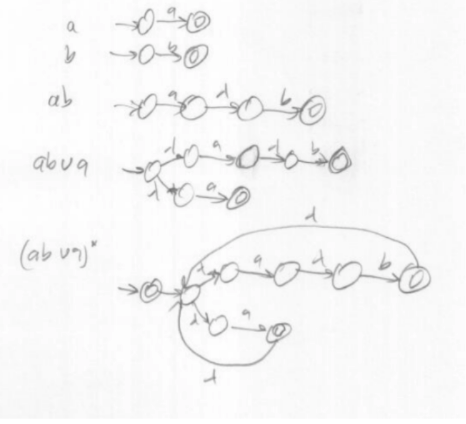
\includegraphics[width=\textwidth]{retonfa}


\textbf{FA to Regular Expression}

\emph{Steps}:

\begin{enumerate}

  \item Start new start and accept states
  \item Rip nodes out untill only the start and accept states are left.
  \item To rip a node out, write down the ``in'' and ``out'' for the rip node
\end{enumerate}


\textbf{Example}

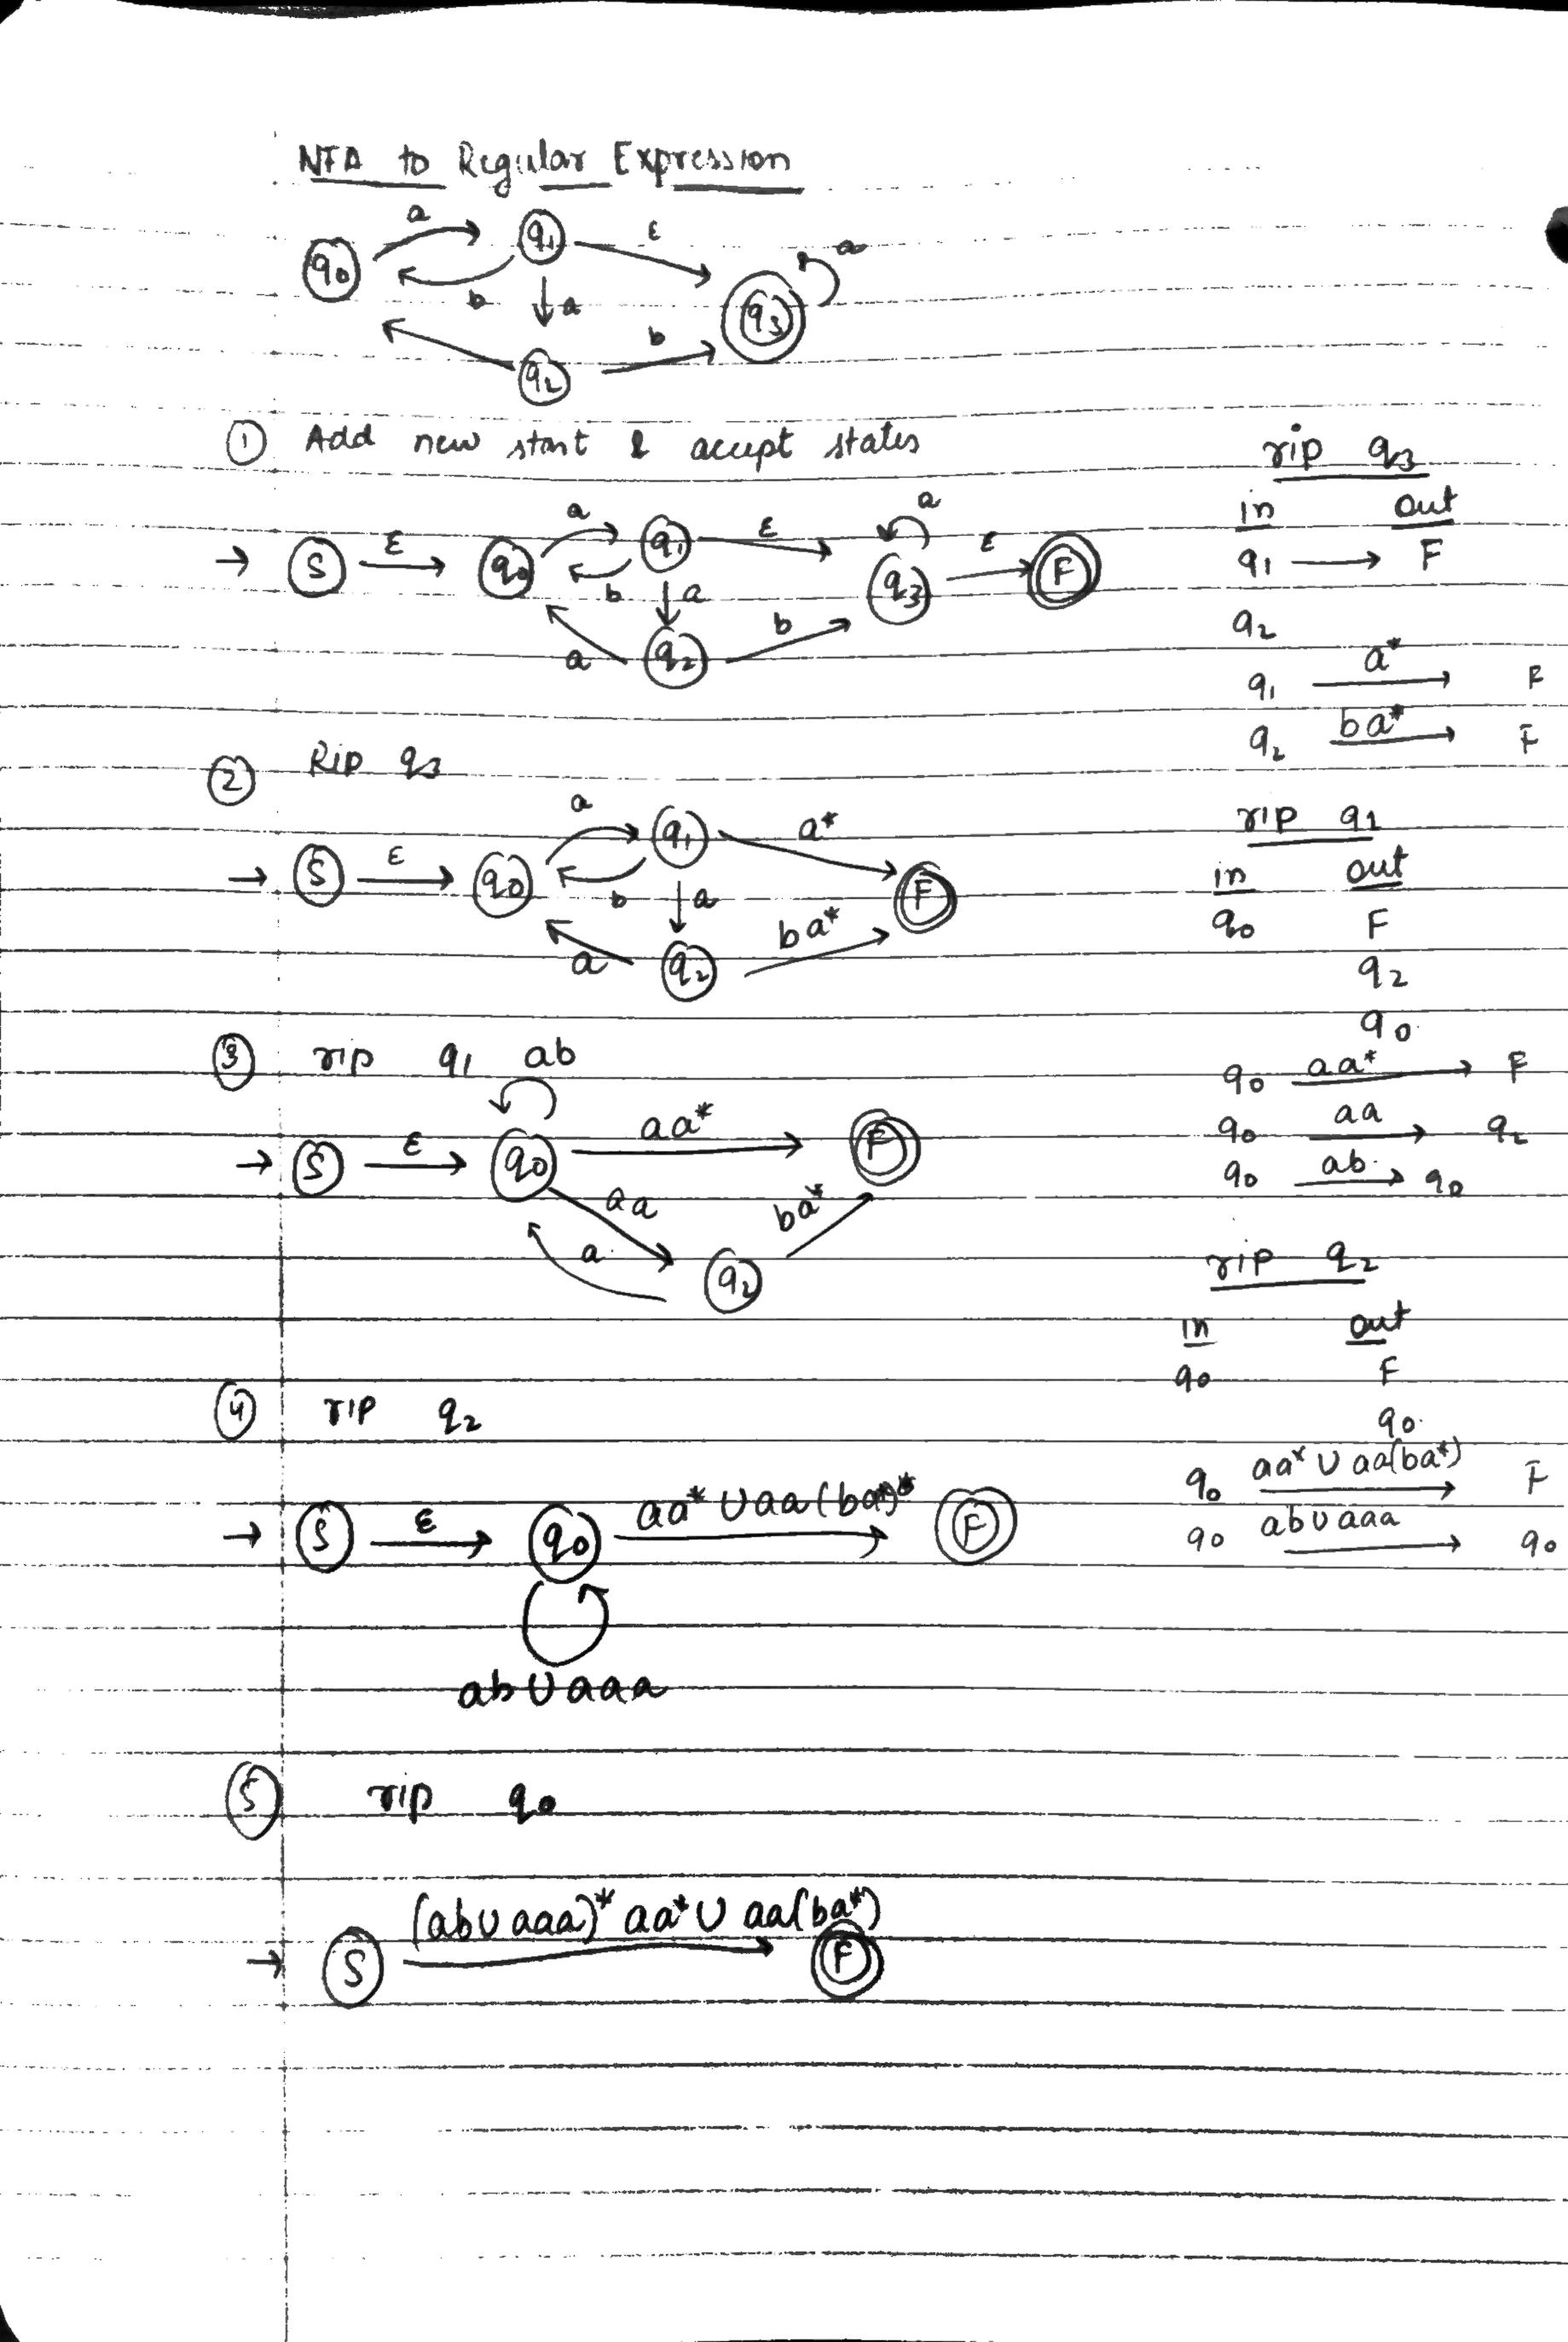
\includegraphics[width=\textwidth]{fatore}


\section{Limits of Finite State Computation}

\textbf{Pumping Lemma for Regular Languages}

if $L$ is regular, then there must be some length $p$ s.t any sufficiently long string $w\in L$, $|w| \ge p$ can be split as $w = xyz$ where:

$|y| > 0$ ($y$ can't be $\epsilon$)

$|xy| \le p$

$xy^{i}z \in L$ for all $i \ge 0$ (i.e $L(xy^{*}z) \subseteq L$)

For sufficiently long strings, there is always a substring y that is arbitrarily repeatable.

\chapter{Context-Free Languages}

\section{Pushdown Automata}

\textbf{Definition} $M = (Q,\Sigma, \Gamma, \delta, q_{0}, F)$ where

$Q$ finite set of states

$\Sigma$ finite input alphabet

$\Gamma$ finite stack alphabet

$\delta: Q\times \Sigma_{\lambda} \times \Gamma_{\lambda}\to \{Q,\Gamma_{\lambda}\}\cup \emptyset$

$q_{0}$ start state

$F\subseteq Q$ set of accepting states


\textbf{Example}


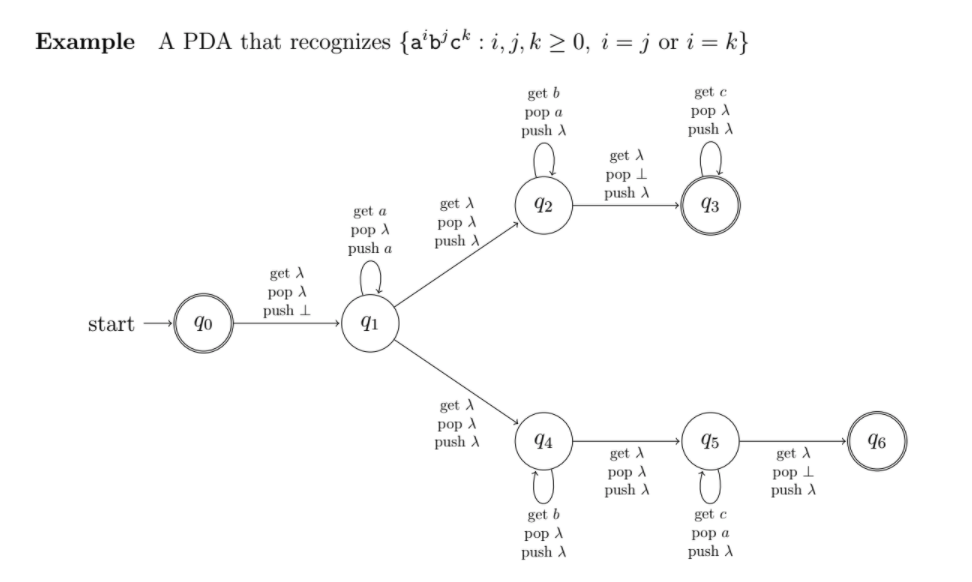
\includegraphics[width=\textwidth]{expda}



\section{Context-Free Grammar}

\textbf{Definition} A \emph{context free grammar} is defined as $G=(V,\Sigma, R,S)$ where

$V$ is the finite set of Variables (``non terminals'')

$\Sigma$ is the finite alphabet (``terminals'')

$R$ is the set of finite rules

$S$ is the start variable
\end{document}
